\section{Results and Analysis} \label{sec:results}
% 1. Accuracy (F1 + MCC) auf SICK und eSNLI einzeln nach Kategorien
% 2. Auf Bias überprüfen: Vergleich vom Modell für wichtig erachtete Token mit von Menschen als wichitg erachtete Tokens
% Visualisierungen:
% - Confusion Matrix (Gentrennt nach Phänomenen)
% - Tabellen Interpretability Metriken (siehe ferret)
In this section the results of our experiments are described and thoroughly analyzed. The results are grouped according to the hypotheses they support.

\subsection{Testing H1}
To test the knowledge contained in \acp{PLM}, we devise prompts that allow for \ac{NLI} predictions, as described in \autoref{sec:meth:probing}. The results obtained using the prompting methods are shown in \autoref{tab:res:prompting}. The word group chosen a priori from the list of discourse markers performs best in F$_1$-Score and second best in \ac{MCC}. The simple word group performs worst in \ac{MCC} but second best in F$_1$-Score. The tuned word group performs best in \ac{MCC} and slightly worse than the simple word group in F$_1$-Score. The difference in F$_1$-Score between a priori and the other word groups is far bigger than the gaps in the \ac{MCC} scores. As the discrepancy is great, we added a metric, the balanced accuracy, to the evaluation that should also be better for imbalanced data than the F$_1$-Score and sometimes more informative than the \ac{MCC} \cite{mccBad}. The balanced accuracy is calculated as the macro-average of the true positive rate of each class \cite{bacc}. Looking at the results in the additional metric, they confirm the ranking obtained by using the \ac{MCC} values. Using this additional fact, we conclude that the \ac{MCC} values are more trustworthy than the F$_1$-Scores for this task.
\begin{table}[ht!]
    \centering
    \caption{Prediction performance when using prompting with different word groups on the \acs{SICK} dataset. The best result is shown in \textbf{bold} and the second-best is \underline{underlined}.}
    \begin{tabular}{l c c c}
        \toprule
        \multicolumn{1}{c}{Word Group} & \acs{MCC} & $\text{F}_1$ & BAcc\\
        \midrule
        A Priori & $\underline{25.51}\%$ & $\mathbf{54.31\%}$ & $\underline{54.11}\%$ \\
        Simple & $20.56\%$ & $\underline{34.40\%}$ & $45.67\%$ \\
        Tuned & $\mathbf{29.11\%}$ & $34.08\%$ & $\mathbf{55.73\%}$\\
        \bottomrule
    \end{tabular}
    \label{tab:res:prompting}
\end{table}

Looking at the resulting \ac{MCC} scores, we can see the expected ordering: The a priori chosen word group is better than the simple words that do not fit into the sentence and the tuned words perform best, as they are tuned on \ac{MultiNLI} to perform better. Interestingly, all approaches, even the simple approach, perform much better than random, which would be an \ac{MCC} of $0$. Nonetheless, compared to the \ac{MCC} score of the fine-tuned model, which is $49.49\%$, the results of using prompting are far worse, even when specifically tuning the prompt words.

\subsection{Testing H2}
\begin{figure}[ht]
    \centering
    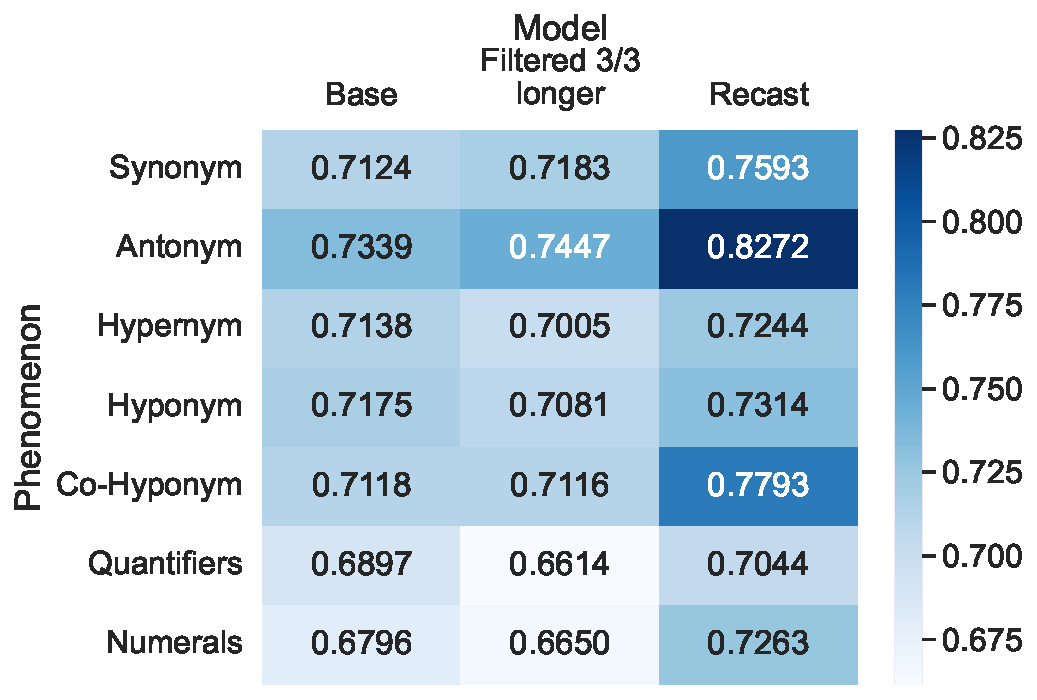
\includegraphics[width=0.9\columnwidth]{./images/metric_heatmaps_phenomena/all_words/base_filtered_recast_matthews_correlation.pdf}
    \caption{\ac{MCC} scores for the models trained on different datasets separated by linguistic phenomena}
    \label{fig:metric-heatmap-phenomena-mcc}
\end{figure}

Figure~\ref{fig:metric-heatmap-phenomena-mcc} depicts the \acs{MCC} scores for our base model separated by linguistic phenomena. As can be seen in the figure, there are disparities between different phenomena. Antonyms, quantifiers and numerals have the largest disparities of $\geq 0.1$. The base model performs best on the phenomenon of antonyms while performing worst on numerals and quantifiers.

Disparities between phenomena indicate a bias of the model towards certain phenomena. As can be seen in \autoref{fig:metric-heatmap-phenomena-mcc}, the base model performs significantly differently when antonyms, quantifiers or numerals occur.

Analyzing the bias metrics of the model for different linguistic phenomena, we focus on \ac{LIME} as the explanation method of choice. \ac{LIME} has the best faithfulness results across all linguistic phenomena and faithfulness metrics and by a significant margin in many cases. We can see the plausibility metrics obtained using \ac{LIME} in \autoref{tab:res:bias_finetuned}. The complete bias metrics can be found in \autoref{sec:bias_plots}, including all explainers and their faithfulness scores.

\begin{table}[ht!]
    \centering
    \caption{Plausibility results obtained using \ac{LIME} as the explainer for different linguistic phenomena.}
    \begin{tabular}{l c c c}
        \toprule
        \multicolumn{1}{c}{Phenomenon} & \acs{AUPRC} & F$_1$ & \acs{IOU}\\
        \midrule
        Synonyms & $52.58\%$ & $38.50\%$ & $25.57\%$ \\
        Antonyms & $68.08\%$ & $47.68\%$ & $33.23\%$ \\
        Hypernyms & $51.08\%$ & $37.05\%$ & $24.33\%$ \\
        Hyponyms & $50.24\%$ & $36.52\%$ & $23.94\%$ \\
        Co-Hyponyms & $53.56\%$ & $39.86\%$ & $26.57\%$ \\
        Quantifiers & $51.33\%$ & $38.26\%$ & $24.87\%$ \\
        Numerals & $50.22\%$ & $37.55\%$ & $25.02\%$ \\
        \bottomrule
    \end{tabular}
    \label{tab:res:bias_finetuned}
\end{table}

Analyzing the plausibility metrics, they are all in the same range except for antonymy. The results on antonymy are far better than on other phenomena, indicating that the model has a far better understanding of the entailment patterns of antonymy. This is indeed unsurprising, as antonyms often indicate contradictions, which is an easy pattern to learn. More complicated patterns such as the ones by quantifiers and numerals have worse plausibility results. Interestingly, the plausibility is worst for hyponymy. As all of those concepts are interlinked, but classification performance is a lot worse for quantifiers and numerals, the bias is inferred to be the worst for those phenomena. As quantifiers can show complex entailment patterns because of their monotonicity properties, we further focus our analysis on quantifiers.

Figure~\ref{fig:ferret-sample} shows the explanations for the fine-tuned model's classification of a sample from the validation split of the \ac{e-SNLI} dataset obtained using ferret \cite{ferret}. It can be seen that the meaning of the quantifiers in this sample is not considered by the model: The usage of quantifiers in this sample makes it a contradiction but the model attaches high importance only to the quantifier \enquote{all} whereas \enquote{several} has very low importance to the model. The existence of such samples where the model only poorly captures the importance of quantifiers shows that the model is biased after fine-tuning on \ac{MultiNLI}.

\begin{figure*}[t!]
    \centering
    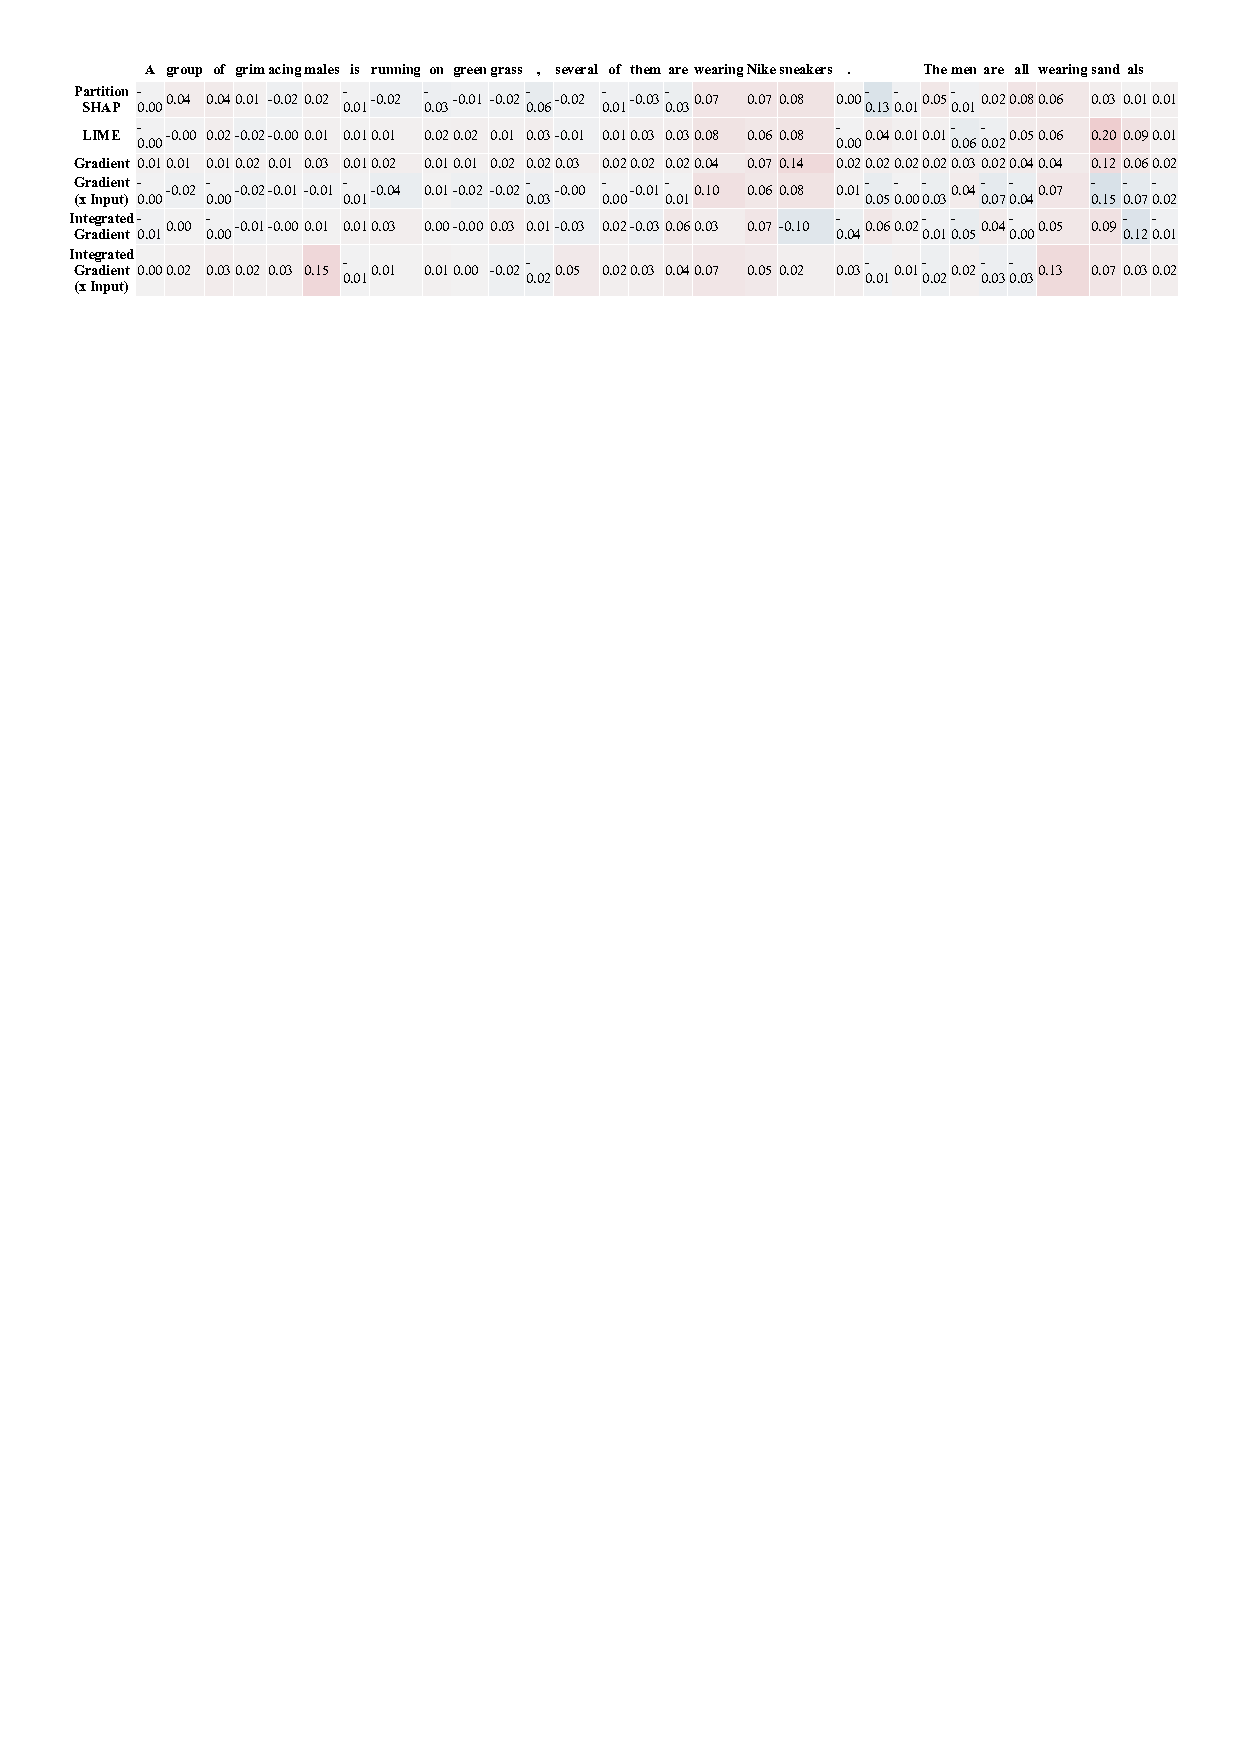
\includegraphics[width=\textwidth]{./images/ferret_sample.pdf}
    \caption{Example of a bad explanation}
    \label{fig:ferret-sample}
\end{figure*}

\subsection{Testing H3}
Figure~\ref{fig:metric-heatmap-phenomena-mcc-hyponly} depicts the \ac{MCC} scores separated by linguistic phenomena for our model trained on different datasets as described in \autoref{sub:experiments-h4} to show the different predictive performance of the models. The results for the hypothesis-only model were measured on the validation-matched split of \ac{MultiNLI}.

\begin{figure}[h!]
    \centering
    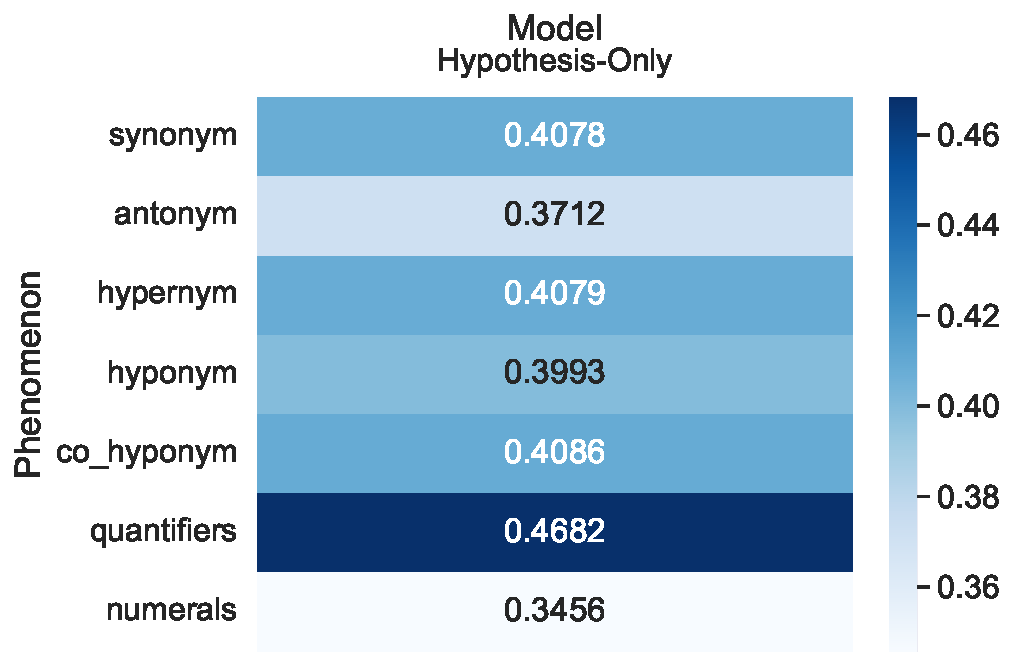
\includegraphics[width=0.9\columnwidth]{./images/metric_heatmaps_phenomena/important_words/hypothesis_only_matthews_correlation.pdf}
    \caption{Matthews Correlation Coefficients for the model trained on different datasets separated by linguistic phenomena}
    \label{fig:metric-heatmap-phenomena-mcc-hyponly}
\end{figure}

In general, the hypothesis-only model shows the expected poor performance: For the phenomena of synonym, hypernym, hyponym and co-hyponym the \ac{MCC} is around $0.4$. The exceptions are antonym, quantifiers and numerals. The model performs particularly poorly on samples that contain antonyms and even worse for numerals. This behavior can be explained by the distribution of phenomena in the dataset shown in \autoref{tab:mnli:phenomena}: Antonyms are found in only $18874$ samples in the training split of \ac{MultiNLI} and numerals only in the hypotheses of $38168$ samples. This makes them the two rarest phenomena in the dataset. 

\begin{table}[ht]
    \centering
    \caption{Phenomena distribution of the hypothesis of the training split of \ac{MultiNLI}}
    \small
    \begin{tabular}{l r}
        \toprule
        \multicolumn{1}{c}{Phenomenon} &  \multicolumn{1}{c}{Number of Samples} \\
        \midrule
        Synonym & $339763$ \\
        Antonym & $18874$ \\
        Hypernym & $117645$ \\
        Hyponym & $124984$ \\
        Co-Hyponym & $381690$ \\
        Quantifier & $48526$ \\
        Numeral & $38168$ \\
        \bottomrule
    \end{tabular}
    \label{tab:mnli:phenomena}
\end{table}

Also comparably rare are samples which contain quantifiers. Nevertheless, the model performs best on samples with an \ac{MCC} of about $0.46$. Since the model cannot possibly determine the meaning of the quantifier for the classification without knowledge of the premise this result is a clear indicator of a bias in the samples that contain quantifiers.

\subsection{Testing H4}
\begin{table}[ht!]
    \centering
    \caption{Prediction performance of our fine-tuned models on the \acs{SICK} dataset. The best result is shown in \textbf{bold} and the second-best is \underline{underlined}.}
    \begin{tabular}{l c c}
        \toprule
        \multicolumn{1}{c}{Model} & \acs{MCC} & $\text{F}_1$ \\
        \midrule
        Base & $49.49\%$ & $56.60\%$ \\
        Hypothesis-Only\tablefootnote{Average of three runs with different seeds} & $14.13\%$ & $40.02\%$ \\
        Filtered $2/3$ & $46.21\%$ & $54.12\%$ \\
        Filtered $2/3$ longer & $36.17\%$ & $52.85\%$ \\
        Filtered $3/3$ & $48.73\%$ & $56.94\%$ \\
        Filtered $3/3$ longer & $\mathbf{52.31\%}$ & $\mathbf{62.04\%}$ \\
        Ensembled & $\underline{51.65\%}$ & $\underline{59.88\%}$ \\
        Recast & $45.33\%$ & $51.64\%$ \\
        \bottomrule
    \end{tabular}
    \label{tab:res:finetuned}
\end{table}

To test this hypothesis, we trained multiple models and evaluated their predictive performance in general and further analyzed the best model. The predictive performance of all models can be seen in \autoref{tab:res:finetuned}, the names follow the names of the datasets introduced in \autoref{sec:experiments}. In this case, a high correlation between the F$_1$-Score and \ac{MCC} can be seen, so we do not need to consult additional metrics. The differences in \ac{MCC} are bigger and the \ac{MCC} was more meaningful when comparing the results of the different prompting methods, therefore we mainly analyze the \ac{MCC} scores.

Unexpectedly, the filtered models perform worse than the base fine-tuned model, even though the data quality should be better. As the models trained on the filtered datasets have been trained for fewer iterations in three epochs, we interpret the inferior results as being because of less training. When evaluating the models trained for more epochs, we can see an improvement for \enquote{Filtered 3/3} and deterioration for \enquote{Filtered 2/3}. This result is only slightly unexpected and can be attributed to \enquote{Filtered 2/3} being more harshly filtered and therefore have even fewer samples which cannot be balanced out by the higher data quality achieved by filtering biased samples more easily. \enquote{Filtered 3/3} shows better performance when trained longer, which indicates it providing a better tradeoff between data quality and data quantity. Therefore, we further analyze \enquote{Filtered 3/3 longer} and use it to compare to the ensembled model.

The ensembled model performs better than the baseline and slightly worse than the filtered model trained longer. This indicates that bias is successfully mitigated during training, as predictive performance on the less biased out-of-domain evaluation set is improved. The performance is still slightly better for the filtered model, we further analyze that instead of the ensemble.

Figure~\ref{fig:metric-heatmap-phenomena-mcc} depicts the \ac{MCC} scores separated by linguistic phenomena for the filtered model compared to the base fine-tuned model. We can see slightly improved performance for antonyms with harshly decreased performance for quantifiers and similar performance for all other phenomena. The decreased performance for quantifiers can be explained by the hypothesis-only model being more accurate on quantifiers and therefore more examples of quantifiers being discarded as biased during filtering. The decreased performance might be explained by either fewer samples of this phenomenon existing after filtering or the evaluation set having the same biases as the training set and thus decreased performance for it that would not exist for a less biased dataset. The increased performance on antonyms but decreased performance on numerals is surprising, as both have poor prediction performance for the hypothesis-only model and thus should not be filtered too much. We interpret that result as random noise or just a general decrease in bias that is randomly effective for antonyms but is not for numerals. Nonetheless, the filtering is beneficial for overall prediction performance, which can be explained by samples not being detected as part of any of our phenomena.

% TODO: description of bias plots

\subsection{Testing H5}
To test this hypothesis the predictive performance of the recast model has been tested on both the \ac{SICK} dataset and the \ac{e-SNLI} dataset.

The results obtained on the \ac{SICK} dataset can be seen in \autoref{tab:res:finetuned}. Unexpectedly, the performance of the model on the \ac{SICK} dataset dropped significantly compared to the base finetuned model both in terms of the \ac{MCC} and F$_1$-Score. This can be explained by the fact that both \ac{e-SNLI} and \ac{MultiNLI} are variants of the \ac{SNLI} dataset and are therefore rather similar to each other. In contrast, \ac{SICK} is from a completely different domain and was specifically constructed to reveal issues with crowdsourced datasets such as \ac{e-SNLI} and \ac{MultiNLI}.

Figure~\ref{fig:metric-heatmap-phenomena-mcc} depicts the result of the recast model on the \ac{e-SNLI} dataset per linguistic phenomenon compared to the other models. The model's performance on samples that contain quantifiers and have been determined to be biased has indeed been improved by the addition of the recast data compared to the base finetuned model. We interpret this as a result of decreased bias in the quantifier samples caused by the additional recast data.

Interestingly, also the performance on all other linguistic phenomena has increased, but most drastically on antonyms on which the model's performance increased by almost ten percentage points. Also on all other linguistic phenomena, the model's performance has increased by at least two percentage points. This behavior can be explained by the increased amount of training data also showing examples of other linguistic phenomena.
